This section accounts for the dataset used and the data pre-processing assumptions made for usability, we also visualize the datasets used. In section \ref{sec:ddsc}, we make a complete outline of the algorithm which is the basis for this thesis. Lastly, in section \ref{sec:implementation}, we review what has been implemented in detail and what tools have been.


\subsection{Dataset}

In this paper, the Pecan Street data \cite{pecan} has been solely used. The reason is that most of the current datasets include as much detail, but lack a vast number of houses, which is needed in order for a deep learning to train itself.

\subsection{Data pre-processing}
\label{sec:prep}
If there is much irrelevant and redundant information present or noisy and unreliable data, then knowledge discovery during the training phase is more difficult. Data preparation and filtering steps have taken considerable amount of processing time. The process has included cleaning, normalization, transformation of the dataset, where the end product have been the final training set.

% - different approaches to the problem
The data that has been chosen for creating the training and testing set have been from the year 2014 and 2015. The raw data contain more than 8 billion readings from different appliances in 689 houses. However the problem with most data is incompleteness. The appliances that have been taken into consideration have been; air, furnace, dishwasher, refrigerator and the summed values of the other appliances called miscellaneous category, for more detail visit \href{http://www.pecanstreet.org/}{Pecan Street Inc}. These appliances were chosen due to the lack of information, investigating the dataset revealed that almost 80\% of the values were not present for most monitored appliances. Out of the chosen appliances, a house was taken into account if it had missing values of more than one appliance for each hour. 

For treating missing values we assuming that appliances run as a constant fashion, meaning that we interpolate the nearest value from the previous reading to complete the dataset. Below we find energy readings of the whole-home usage of electricity in the dataset.

\begin{figure}[H]
	\centering
	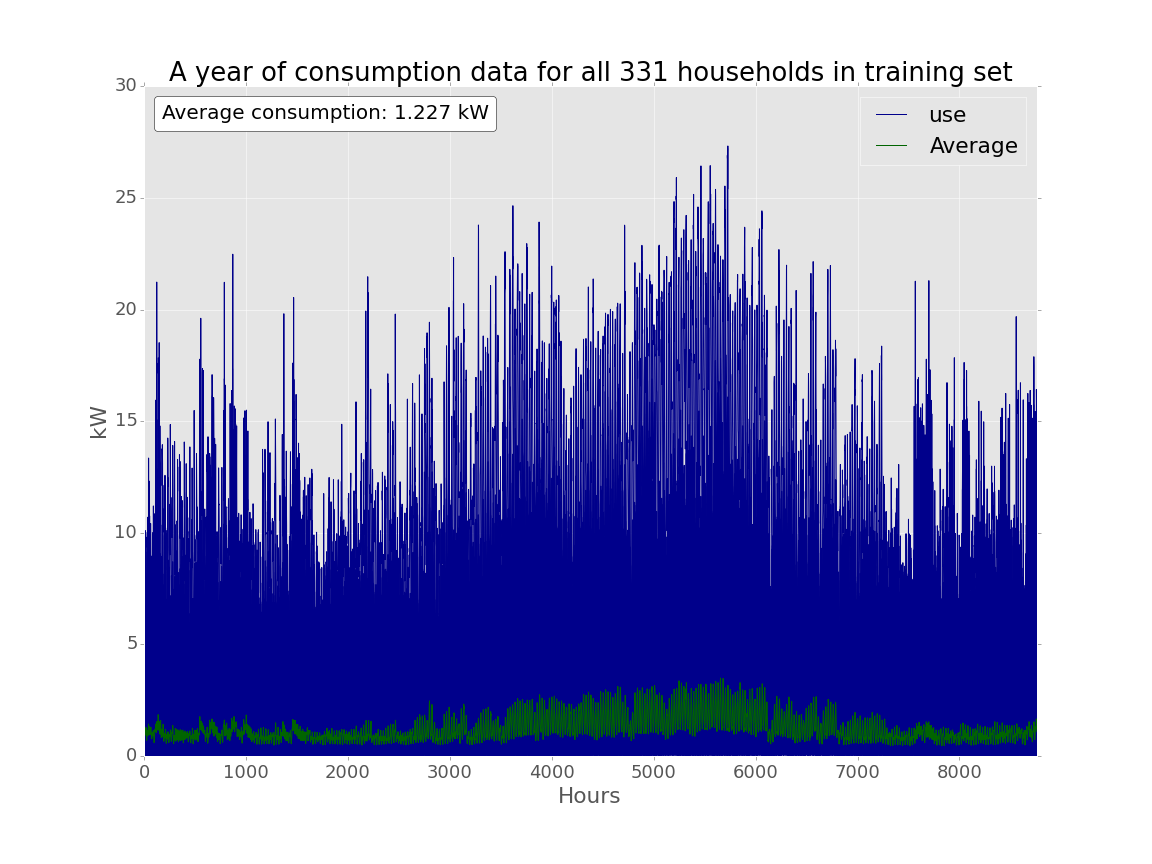
\includegraphics[scale=0.30]{./figures/houseuse}
	\caption{Training households, 2014}
	\label{fig:houseuse}
\end{figure}

As seen from the figure \ref{fig:houseuse}, some houses end up using almost 10 times more elecricity than the average household. These households have an impact to focus less on the more generalized households. Presumably these households are not of interest for Greenely or the generalized result in which we would want to classify. Here the assumption has been that these households are more of industrial size, although not nearly enough power consumption to be compared to, but acting more of a reference for which households have been investigated.

\begin{figure}[H]
	\centering
	\begin{minipage}{.5\textwidth}
		\centering
		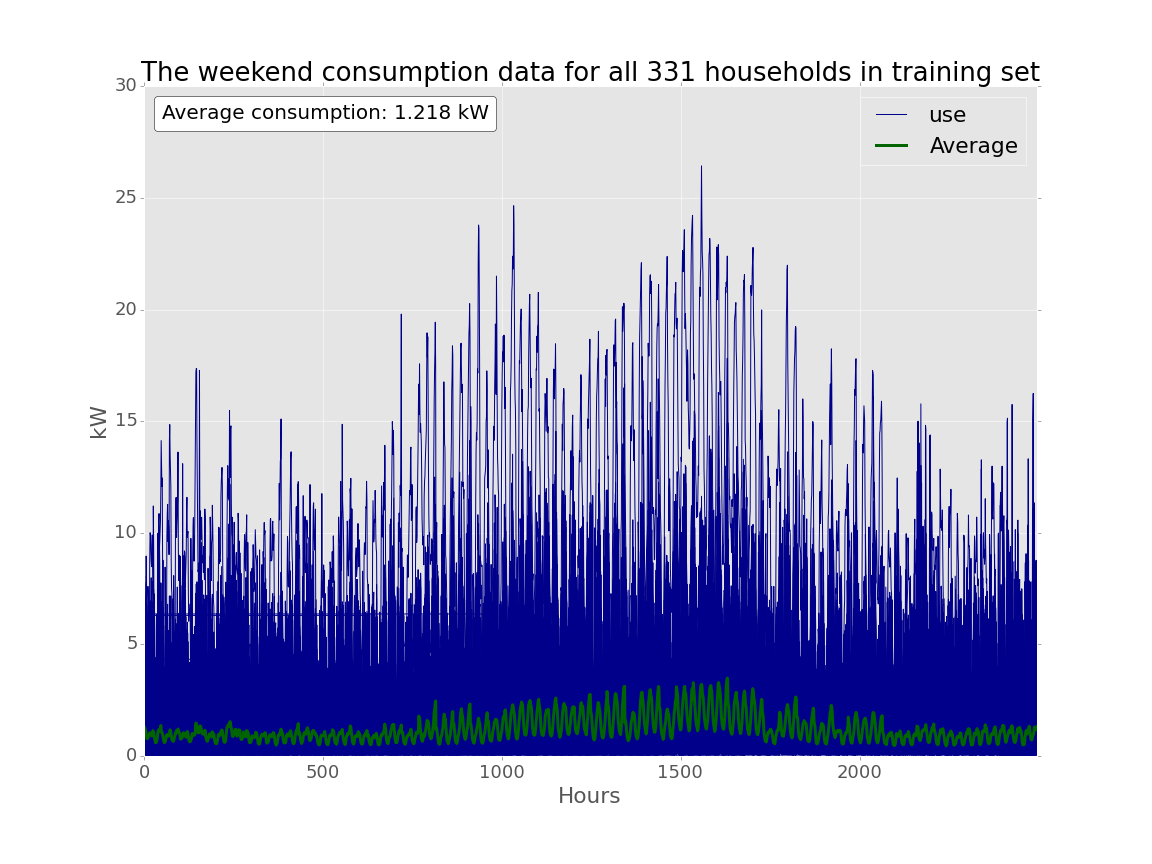
\includegraphics[scale=0.19]{./figures/weekendhouseuse}
		%\label{fig:test6}
	\end{minipage}%
	\begin{minipage}{.5\textwidth}
		\centering
		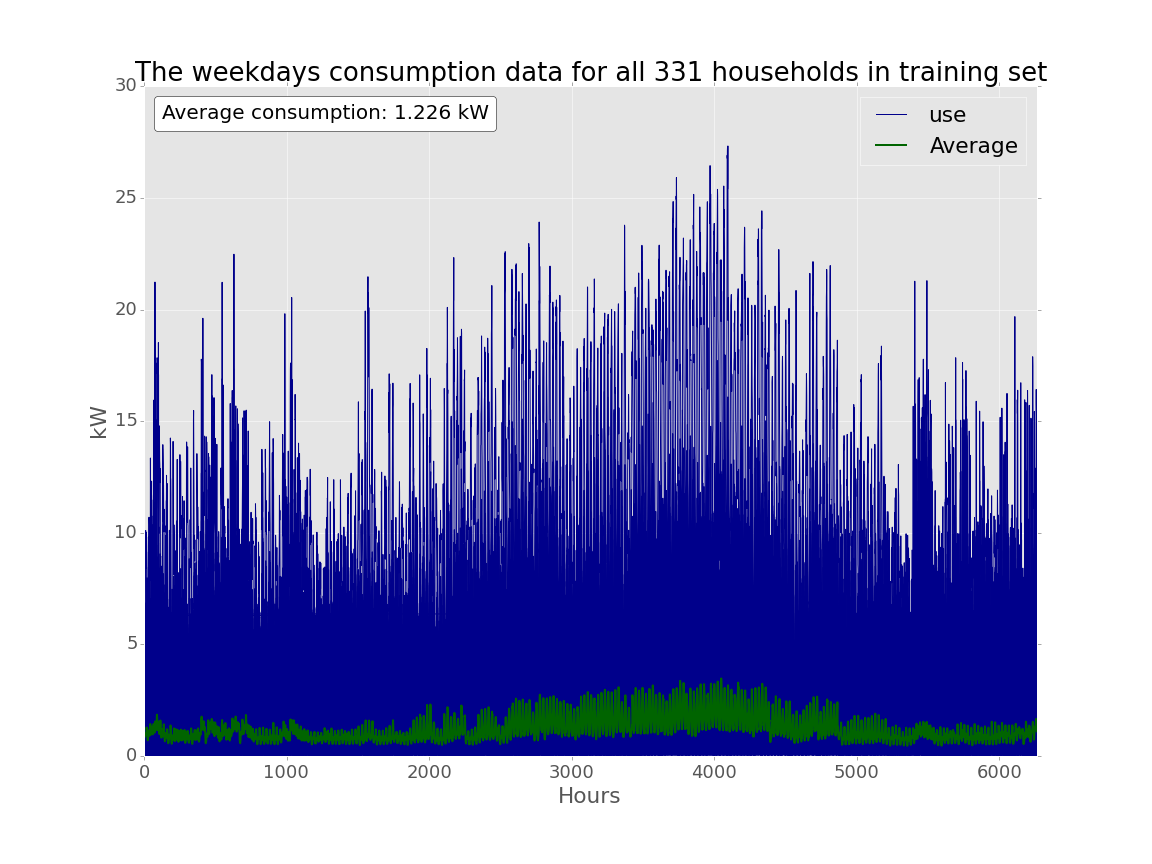
\includegraphics[scale=0.19]{./figures/weekdayshouseuse}
		%\label{fig:test5}
	\end{minipage}
	\caption{This figure shows two plots representing the weekday and weekend datasets. The datasets are compressed of a whole year of weekdays and weekends respectively. The left plot have values for all the hours of the weekends for a year 2496 hours. The right plot consists of hourly readings of 6240 hours.}
	\label{fig:weekend_day}
\end{figure}

From the figure above \ref{fig:weekend_day}, we can see that the left plot which has the weekends, consists of peaks of consumption. In comparison with the right plot, where we have a more consistent behaviour of the household consumption. However, we note that energy consumption show that it is not significant enough to take into consideration. We conclude that the algorithm could find better shapes within the data when the dataset has been split, however there will probably be no seen affect from the energy consumption.

\begin{figure}[H]
	\centering
	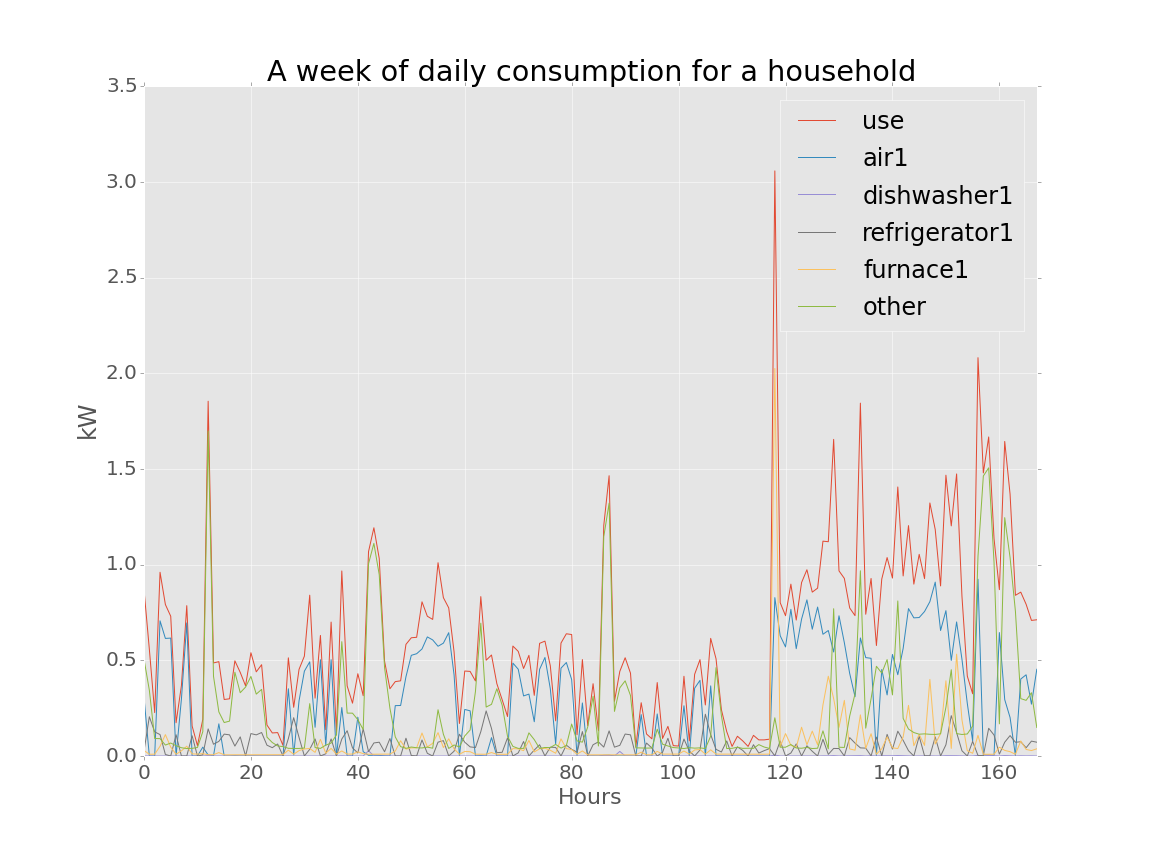
\includegraphics[scale=0.30]{./figures/weekconsump}
	\caption{A week of the consumption data for the appliances and whole-home usage}
	\label{fig:weekconsump}
\end{figure}

The figure shows consumption of the considered appliances. Pecan Street Inc's dataset is a great source of energy consumption data, however they have made a choice of registering average consumption of the particular appliance during that interval, with the aim that; if a refrigerator has been consuming one kilowatt per minute for 10 min and then gets turned off, it will be represented as $\frac{1}{10}$ instead of $\frac{1}{60}$, which could make the observation-based method flawed, as the assumption of precise measurements is the basis of the algorithm that Kotler et. al. presented \cite{DDSC}. 

\begin{figure}[H]
	\centering
		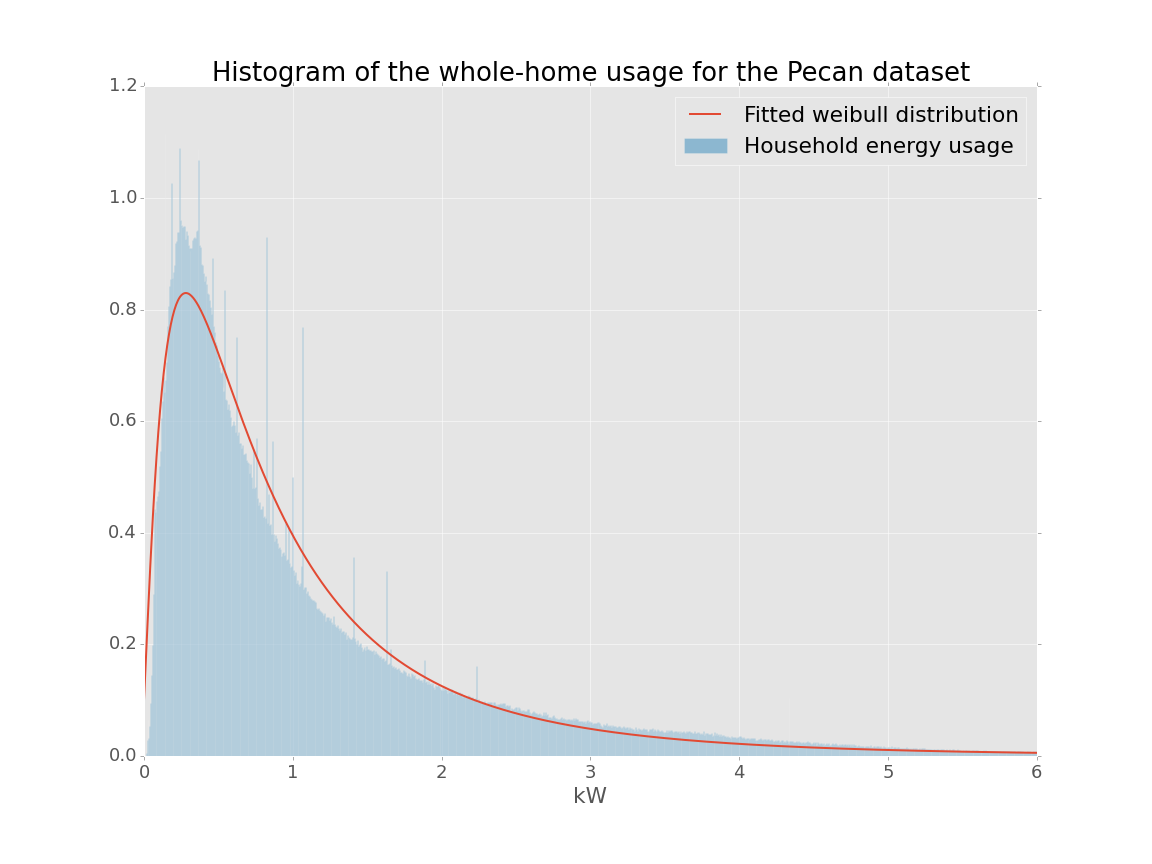
\includegraphics[scale=0.30]{./figures/new_histusage}
		\caption{Histogram of the household usage.}
		\label{fig:histuseage}
\end{figure}

The histogram in figure \ref{fig:histuseage} is presented to show that the usual consumption is substantially around the values 0.2 to 0.8 kW per hour. This is what Energy Information Administration \href{http://www.eia.gov/tools/faqs/faq.cfm?id=97&t=3}{EIA} presented in 2013 \cite{eia}, where they present the average consumption of an American household to 10,908 kilowatthours (kWh) which in turn corresponds to:

\begin{equation*}
	10.908 \textbf{kWh} / (24\times365) \textbf{h} = 1.245205479 \textbf{kW}
\end{equation*}

The average consumption for the Pecan Street households is 1.2244009446607182 \textbf{kW}, in the regard of average consumption the dataset can be seen as a good representation for a general household within the United States. Interesting to note is that the data can be fitted to a Weibull distribution, which has been used for providing dummy data.

\newpage
% --
\subsection{Discriminative Disaggregation via Sparse Coding}
\label{sec:ddsc}
This approach was presented in 2011 by J. Kolter MIT and Batr, Y.Nh from Stanford in \cite{DDSC}. It is based on improvements of single-channel source separation and enable a sparse coding algorithm to learn a model of each device's power consumption over a typical week. These learned models are then combined to predict the power consumption of different devices in previously unseen homes, using only their aggregate signal. Typically these algorithms have been used in audio signal separation, which usually has high temporal resolution (precision of measurement w.r.t. time) in contrast to low-resolution energy disaggregation; which impose new challenges within the field. Their algorithm shows an improvement of discriminatively training sparse coding dictionaries for disaggregation tasks. More specifically, they formulate the task of maximizing disaggregation as a structured prediction problem. 

The sparse coding approach to source separation, which forms for the basis for disaggregation, is to train separate models for each individual class $\mathbf{X}_i \in \mathbb{R}^{T\times m}$, where $T$ is the number of samples (hours in the given timeperiod) and $m$ is the number of features (households included) then use these models to separate an aggregate signal. Formally, sparse coding; models the $i$th data matrix using the approximation $\mathbf{X}_i \approx \mathbf{B}_i\mathbf{A}_i$ where the columns of $\mathbf{B}_i \in \mathbb{R}^{T \times n}$ contain a set of $n$ basis functions, also called the dictionary, and the columns of $\mathbf{A}_i \in \mathbb{R}^{n \times m}$ contain the activations of these basis functions, see section \ref{sec:scnn} for more detail. The data input is describe below:

\begin{itemize}
	\item{We define one class (e.g. heater) $\mathbf{X}_i \leftarrow 1,\dots,
		k$}
	\item{Where $\mathbf{X}_i \in \mathbb{R}^{T \times m}$, ex: week $T=24\times7=168$ of $m$ houses}
	\item{\textbf{One} aggregated household $\bar{\mathbf{X}} \leftarrow \sum_{i:k} \mathbf{X}_i$}
	\item{Assuming we have individual energy readings $\mathbf{X}_1,\dots,\mathbf{X}_k$}
	\item{Sparse encode $\mathbf{A},\mathbf{B}$ such that $(n \gg m,T)$}
	\item{Goal: test with new data $\bar{\mathbf{X}}'$ to components
		$\mathbf{X}_1',\dots,\mathbf{X}_k'$}
\end{itemize}

Sparse Coding additionally imposes the constraint that the activations $\mathbf{A}_i$ be sparse, i.e., that they contain mostly zero entries. This allows for learning \textit{overcomplete} sets of representations of the data (more basis functions than the dimensionality of the data, $n \gg m,T$). This makes sparse coding interesting for the field of energy disaggregation since the input data (energy consumption) is inherently positive. They also impose that the activations and dictionaries (bases) be non-negative, presented by \cite{hoyer} as non-negative sparse coding, see section \ref{sec:nnsc} for more detail. The non-negative sparse coding objective

\begin{equation}
\min_{\mathbf{A} \geq 0} \norm{\mathbf{X}_i - \mathbf{B}_i\mathbf{A}}_F^2 + \lambda \sum_{p,q} \mathbf{A}_{pq} \quad \text{subject to} \quad \norm{\mathbf{b}_i^{(j)}}_2 \leq 1, j=1,\dots,n
\end{equation}

where $\mathbf{X}_i,\mathbf{A}_i$ and $\mathbf{B}_i$ are defined as above, while $\lambda \in \mathbb{R}_+$ is a regularization parameter and norms defined as in beginning of section 2 \ref{sec:theoretical}. The sparse coding optimization problem is convex for each optimization-variable whilst holding the other variable fixed. The most common technique is to alternate between minimizing the objective over $\mathbf{A}_i$ and $\mathbf{B}_i$ \cite{DDSC}.

When the representations have been trained for each of the classes (appliances), we concatenated the bases to form a single joint set of basis functions and solve a disaggregation for a new aggregate signal $\bar{\mathbf{X}} \in \mathbb{R}^{T\times m'}$ using the procedure presented below. 

\begin{equation}
\label{eq:f}
\begin{aligned}
\hat{\mathbf{A}}_{1:k}  & = \arg \! \min_{\mathbf{A_{1:k}} \geq 0} \norm{\bar{\mathbf{X}}-\left[\mathbf{B}_1 \cdots \mathbf{B}_k\right]  
		\begin{bmatrix}
		\mathbf{A}_1 \\
		\vdots \\
		\mathbf{A}_k
		 \end{bmatrix}
	}_F^2 + \lambda \sum_{i,p,q}(\mathbf{A}_i)_{pq} \\
 & \vcentcolon= \arg \! \min_{\mathbf{A_{1:k}} \geq 0} F(\bar{\mathbf{X}},\mathbf{B}_{1:k},\mathbf{A}_{1:k})
\end{aligned}
\end{equation}

where $\mathbf{A}_{1:k}$ is denoted as $[\mathbf{A}_1,\dots,\mathbf{A}_k]$ and we abbreviate the optimization objective as $F(\bar{\mathbf{X}},\mathbf{B}_{1:k},\mathbf{A}_{1:k})$. We then predict the $i$th component of the signal to be 

\begin{equation}
\hat{\mathbf{X}}_i = \mathbf{B}_i \hat{\mathbf{A}_i}.
\end{equation}

The intuition is that if $\mathbf{B}_i$ is trained to reconstruct the $i$th class with small activation, then it should better represent the $i$th portion of the aggregate signal than all other bases $\mathbf{B}_j$ for $j\neq i$. Henceforth they construct a way of evaluating the quality of the resulting disaggregation (\textit{disaggregation error})

\begin{equation}
\label{eq:diserr}
E(\mathbf{X}_{1:k},\mathbf{B}_{1:k}) \vcentcolon= \sum_{i=1}^k \frac{1}{2} \norm{\mathbf{X}_i - \mathbf{B}_i \hat{\mathbf{A}}_i}_F^2 \ \text{s.t.} \ \hat{\mathbf{A}}_{1:k} = \arg \! \min_{\mathbf{A_{1:k}} \geq 0} F\left( \sum_{i=1}^k \mathbf{X}_i,\mathbf{B}_{1:k},\mathbf{A}_{1:k} \right),
\end{equation}

which quantifies the reconstruction process for each individual class when using the activations obtained only via the aggregated signal.

\subsubsection{Structured prediction for Discriminative Disaggregation Sparse Coding}

One of the issues that Andrew Ng and J.Zico Kotler point out, using Sparse Coding, the training is solely done for each appliance at hand when the whole-home consumption from consumers have a large variance, as can be seen in figure \ref{fig:houseuse}. The method revolves around training each individual class to produce a small disaggregation error. It is furthermore hard to optimize the disaggreagtion error direcly over the basis $\mathbf{B}_{1:k}$, ignoring the dependance of $\hat{\mathbf{A}}_{1:k}$ on $\mathbf{B}_{1:k}$, resolving for the activations  $\hat{\mathbf{A}}_{1:k}$ ; thus ignoring the dependance of $\hat{\mathbf{A}}_{1:k}$ on $\mathbf{B}_{1:k}$, which loses much of the problem's structure and this approach performs very poorly in practice.

In their paper they define an augmented regularized disaggregation error objective
\begin{equation}
\label{eq:regerror}
\begin{aligned}
\tilde{E}_{reg}(\mathbf{X}_{1:k},\mathbf{B}_{1:k},\tilde{\mathbf{B}}_{1:k})  & \vcentcolon=  \sum_{i=1}^k \left( \frac{1}{2} \norm{\bar{\mathbf{X}}-\mathbf{B}_i  \hat{\mathbf{A}}_i}_F^2 + \lambda \sum_{i,p,q}(\hat{\mathbf{A}}_i)_{pq} \right) \\
& \text{subject to } \hat{\mathbf{A}}_{1:k} = \arg \! \min_{\mathbf{A_{1:k}} \geq 0} F\left(\sum_{i=1}^k \mathbf{X}_i,\tilde{\mathbf{B}}_{1:k},\mathbf{A}_{1:k}\right),
\end{aligned}
\end{equation}

where the $\mathbb{B}_{1:k}$ bases (referred to as the reconstruction basis) are the same sas those learned from sparse coding while the $\tilde{\mathbf{B}}_{1:k}$ bases (disaggreagtion bases) are discrimintively optimized in order to move $\hat{\mathbf{A}}_{1:k}$ close to $\mathbf{A}_{1:k}^{\bigstar}$, without changing these targets. For more detail regarding this section, see Kotler et.al. page four \cite{DDSC}. Here they describe that we seek bases $\tilde{\mathbf{B}}_{1:k}$ such that (ideally)

\begin{equation}
\mathbf{A}_{1:k}^\bigstar = \arg \! \min_{\mathbf{A_{1:k}} \geq 0} F ( \bar{\mathbf{X}}, \tilde{\mathbf{B}}_{1:k},\mathbf{A}_{1:k}).
\end{equation}

In paper \cite{DDSC} it is noted that many methods can be applied to the prediction problems. They chose a structured prediction algorithm presented in Collins 2005 \cite{collins}. Given some value of the parameters $\tilde{\mathbf{B}}_{1:k}$, we first compute $\hat{\mathbf{A}}$ using equation \ref{eq:f}. The perceptron update with a step size $\alpha$ is now

\begin{equation}
\tilde{\mathbf{B}}_{1:k} \leftarrow \tilde{\mathbf{B}}_{1:k} - \alpha \left( \Delta_{\tilde{\mathbf{B}}_{1:k}} F(\bar{\mathbf{X}},\tilde{\mathbf{B}}_{1:k},\mathbf{A}_{1:k}^\bigstar) - \Delta_{\tilde{\mathbf{B}}_{1:k}} F(\bar{\mathbf{X}},\tilde{\mathbf{B}}_{1:k},\hat{\mathbf{A}}_{1:k} \right)
\end{equation}

or to be more explicit by defining the concatenated matrices $\tilde{\mathbf{B}} = [ \tilde{\mathbf{B}}_1 \cdots \tilde{\mathbf{B}}_k ], \mathbf{A}^\bigstar = [{\mathbf{A}_1^\bigstar}^T \cdots{\mathbf{A}_k^\bigstar}^T ]$ (similar for $\hat{\mathbf{A}}$),

\begin{equation}
\label{eq:4b}
\tilde{\mathbf{B}} \leftarrow \left[ \tilde{\mathbf{B}} - \alpha \left( (\bar{\mathbf{X}} - \tilde{\mathbf{B}}\hat{\mathbf{A}})\hat{\mathbf{A}}^T - (\bar{\mathbf{X}}-\tilde{\mathbf{B}}\mathbf{A}^\bigstar)(\mathbf{A}^\bigstar)^T \right) \right]_+
\end{equation}

In conjuncting with the equation above, we keep the postive values of $\tilde{\mathbf{B}}_{1:k}$ and re-normalize each column to have unit norm (step 4c in DDSC algorithm \ref{alg:ddsc}). 

\subsection{Implementation}
\label{sec:implementation}
The vast increase of interest within Machine Learning and the applications that it can bring in the digitized aged have made it possible for many Open Source libraries used for Sparse Coding. In this thesis \textsc{Python} has been used as a means of implementation. The source code for the implemented algorithms can be found in section \ref{sec:appendix} and the mathematical notation is found below in section \ref{sec:implemented}. Below is a list of libraries connected to Machine Learning using \textsc{Python} and the argumentation behind the libraries chosen.

\begin{itemize}
	\item{NeuroLab, Deep Learning}
	\item{Theano, Deep Learning}
	\item{Statsmodels, Statistical library}
	\item{Scikit-Learn, General Machine Learning \cite{scikit}}
	\item{Librosa, Signal processing library}
\end{itemize} 

Neurolab and Theano are the more low-level deep learning libraries, that provide the users with lots of options, but however needs a great deal of knowledge in both python and deep learning. Statsmodels is a \textsc{Python} module that allows users to explore data, estimate statistical models, and perform statistical tests. We chose to use the standard Machine Learning library \href{www.scikit-learn.org}{Scikit-Learn}  and \href{http://theremin.ucsd.edu/~bmcfee/librosadoc/index.html}{Librosa}. Scikit-Learn is the go to library when it comes to Machine Learning with \textsc{Python} as it provides a whole set of constructs to build from and to test the algorithms, as well as a vast community. The Librosa library was chosen as it exclusively provides a set for signal processing methods. Although the DDSC algorithm relies on standard methods, the libraries provide a means to proven and tested algorithms. J.Zico Kotler et. al. explain that they had space constraints to preclude a full discussion about the implementation details. They however present the algorithms used, as specified from Kotler et. al. \cite{DDSC} the procedure of DDSC we have implemented a coordinate descent for the steps 2a and 4a in algorithm \ref{alg:ddsc} using Scikits module \href{http://scikit-learn.org/stable/modules/generated/sklearn.decomposition.SparseCoder.html#sklearn.decomposition.SparseCoder}{SparseCoder} and using Librosa to decompose for retreiving the activation matrix. They also refer to Hoyer's paper \cite{hoyer} on multiplicative non-negative matrix factorization update to solve step 2b. The algorithm is presented in \ref{alg:nnsc} as non-negative matrix factorization. The step 4b in the algorithm is explained in equation \ref{eq:4b} as a means to update the basis, and is a straight forward implementation.


\subsection{Implemented Algorithms}
\label{sec:implemented}
The source code for the Non-Negative Sparse-Coding algorithm can be found in Appendix \ref{sec:sc_nnsc} and the source code for the Discriminative Disaggregation algorithm can be found in Appendix \ref{sec:sc_dd}.

\subsubsection{Non-Negative Sparse-Coding}
\label{alg:nnsc}
\begin{algorithm}[H]
	\caption{Non-Negative Sparse Coding}

	\SetKwInOut{Input}{input}
	\Input{Solving the problem of equation \ref{eq:nnsc} in the section for Non-Negative Sparse Coding, \ref{sec:nnsc}}
	\begin{algorithmic}[1]
		\Statex{Interate until convergence:}
		\State{Set positive values for $\mathbf{B}^0$ and $\mathbf{A}^0$, and also set $t=0$.}
		\State{a) $\mathbf{B}' = \mathbf{B}^t - \mu(\mathbf{B}^t \mathbf{A}^t-\mathbf{X})(\mathbf{A}^t)^T$.}
		\Statex{b) Set negative values of $\mathbf{A}'$ to zero.}
		\Statex{c) Rescale $\mathbf{B}'$ to unit norm, and then set $\mathbf{B}^{t+1}=\mathbf{B}'$.}
		\Statex{d) $\mathbf{A}^{t+1}=\mathbf{A}^t.*((\mathbf{B}^{t+1})^T\mathbf{A})./((\mathbf{B}^{t+1})^T(\mathbf{B}^{t+1}\mathbf{A}^t+\lambda))$.}
		\Statex{e) Convergence if $\norm{ \mathbf{A}^{t+1} - \mathbf{A}^{t} } < \epsilon$}
		\Statex{f) Increment t.}
		
	\end{algorithmic}
\end{algorithm}

\subsubsection{Discriminative Disaggregation via Sparse Coding}
\label{alg:ddsc}
%
\begin{algorithm}[H]
\caption{Discriminative Disaggregation via Sparse Coding}
\SetKwInOut{Input}{input}
\Input{data points for each individual source $\mathbf{X}_i \in
\mathbb{R}^{T \times m}, i = 1:k,$ regularization $\lambda
\in \mathbb{R}_+$, with gradient step size $\alpha \in \mathbb{R}_+$.}
\begin{algorithmic}[1]
\Statex{  \textbf{Sparse coding pre-training:}}
\Statex{  \hspace{0.2in} 1. Initalize \textbf{B}$_i$, $\mathbf{A}_i \ \geq 0$, scale columns $\mathbf{B}_i$ s.t. $\norm{ \mathbf{b}_i^{(j)}}_2 =1$}
\Statex{ \hspace{0.2in} 2. For each $i=1,\dots,k,$ iterate until convergence: }
\Statex \hspace{0.4in} $\mathbf{A_i} \leftarrow \arg \! \min_{\mathbf{A} \geq 0} \norm{\mathbf{X}_i - \mathbf{B}_i\mathbf{A}}_F^2 + \lambda \sum_{p,q} \mathbf{A}_{pq}$
\Statex \hspace{0.4in} $\mathbf{B}_i \leftarrow  \arg \! \min_{\mathbf{B} \geq 0,\norm{\mathbf{b}^{(j)}}_2 \leq 1} \norm{\mathbf{X}_i - \mathbf{B} \mathbf{A}_i }_F^2$
\Statex \textbf{Discriminative disaggregation training:}
\Statex  \hspace{0.2in} 3. Set $\mathbf{A}_{1:k}^* \leftarrow \mathbf{A}_{1:k},\hat{\mathbf{B}}_{1:k} \leftarrow \mathbf{B}_{1:k}.$
\Statex  \hspace{0.2in} 4. Iterate until convergence:
\Statex \hspace{0.4in} $\hat{\mathbf{A}}_{1:k} \leftarrow \arg \! \min_{\mathbf{A}_{1:k} \geq 0} F\left( \bar{\mathbf{X}},\tilde{\mathbf{B}}_{1:k},\mathbf{A}_{1:k} \right)$
\Statex \hspace{0.4in} $\tilde{\mathbf{B}} \leftarrow \left[ \tilde{\mathbf{B}} - \alpha \left( (\bar{\mathbf{X}} - \tilde{\mathbf{B}}\hat{\mathbf{A}})\hat{\mathbf{A}}^T - (\bar{\mathbf{X}}-\tilde{\mathbf{B}}\mathbf{A}^\bigstar)(\mathbf{A}^\bigstar)^T \right) \right]_+$
\Statex \hspace{0.4in} $\forall \  i,j, \quad \mathbf{b}_i^{(j)} \leftarrow \mathbf{b}_i^{(j)} / \norm{\mathbf{b}_i^{(j)}}_2$
\Statex \textbf{Given aggregated test examples $\bar{\mathbf{X}}'$}
\Statex \hspace{0.2in} 5. $\hat{\mathbf{A}}'_{1:k} \leftarrow \arg \! \min_{\mathbf{A}_{1:k} \geq 0} F(\bar{\mathbf{X}}',\tilde{\mathbf{B}}_{1:k},\mathbf{A}_{1:k})$
\Statex \hspace{0.2in} 6. Predict $\hat{\mathbf{X}}_i' = \mathbf{B}_i\hat{\mathbf{A}}_i'$
\end{algorithmic}
\end{algorithm}